\section{Evaluation}
\label{sec:eval}

\begin{table}[t]
\centering
\small
\begin{tabular}{p{0.15\columnwidth} p{0.75\columnwidth}}
\toprule
\textbf{CPU} & 2$\times$Xeon E5-2650v2~2.6~GHz,\\
        & 16 cores in total after disabling hyperthreading
\\
\midrule
\textbf{RAM} & 64~GB 1.86~GHz DDR3
\\
%\midrule
%\textbf{Disks} & 4 x WDC WD5003ABYX-18WERA0 (500GB, 7200 rpm, RAID5)
%\\
\midrule
\textbf{NIC} & Mellanox FDR CX3 Single port (40~Gbps)
\\
\midrule
\textbf{Switch} & 36 port Mellanox SX6036G (in Ethernet mode)
\\
\midrule
\textbf{OS} & Ubuntu 15.04, Linux 3.19.0-16,\\
        & DPDK~16.11, MLX4~PMD, 1$\times$1~GB~Hugepage
\\
\bottomrule
\end{tabular}
\caption{Experimental cluster configuration. The evaluation was
carried out on a 24 node c6220 cluster on CloudLab. Hyperthreading was
disabled on all nodes. Of the 24 nodes, 1
ran the coordinator, 8 ran one client each, and the rest ran
RAMCloud servers.
}
%Ports
%on the Mellanox MX354A NICs and SX6036G switch were flipped to Ethernet
%mode.
%The DPDK poll mode driver was configured to use the 40 Gbps port
%on the NIC.
%Cloudlab also provides a 1Gbps control network which was
%used for experiment management.}
\label{table:exptconfig}
\end{table}

To evaluate Rocksteady, we focused on five key questions:
\begin{description}
\item[How fast can Rocksteady go and meet tight SLAs?]
  \S\ref{sec:e2e} shows Rocksteady can sustain migration at
    758~MB/s with \nnnth percentile access latency of less than 250~\us.
\item[Does lineage accelerate migration?]
  Lineage and deferred log replication allow Rocksteady to migrate data
    1.4$\times$ faster than synchronous re-replication, while shifting
    load from the source to the target more quickly (\S\ref{sec:e2e}).
\item[What is the impact at the source and target?]
  \S\ref{sec:eval-load}\linebreak{}shows that regardless of workload skew, Rocksteady
    migrations cause almost no increase in source dispatch load, which is the source's
    most scarce resource for typical read-heavy workloads. Background \pulls
    add about 45\% worker CPU utilization on the source, and Rocksteady
    effectively equalizes CPU load on the source and target.
    Dispatch load due to the migration manager on the target is minimal.
\item[Are asynchronous batched priority pulls effective?]
  \S\ref{sec:eval-priopulls} shows that asynchronous priority pulls are
    essential in two ways. First, synchronous priority pulls would increase both
    dispatch and worker load during migration due to the increased number of
    RPCs to the source and the wasted effort waiting for \priopull responses. Second,
    asynchronous batched \priopulls reduce load at the source fast enough to help
    hide the extra load due to background \pulls on the source, which is key to
    Rocksteady's fast transfer.
\item[What limits migration?]
  \S\ref{sec:eval-replay} shows that the source and target can send/consume
    small records at 5.7~GB/s and 3~GB/s, respectively; for small records
    target replay limits migration more than 
    networking (5~GB/s today).
    Target worker cores spend 1.8~to~2.4$\times$ more cycles
    processing records during migration than source worker cores.

%\item[What is the impact of migration on source and target throughput and tail latnecy}]
%  Tunables include: pull size, parallelism (pulls, and replays).
%    (Microbenchmark)
%\item What is rocksteady's impact on the source and destination -
%dispatch and worker load? (Microbenchmark)
%\item How does hash table selectivity impact migration speed?
%(Microbenchmark)
%\item How good is rocksteady at balancing load? Present three
%configurations - only background task, background task + synchronous
%priority pulls, and background task + batched priority pulls with client
%backoffs. Might want to vary the priority of replay and pull rpcs for
%each of these configurations.
%\item How does re-replication speed impact performance after migration?
\end{description}

\subsection{Experimental Setup}
\label{sec:setup}
%K aniraj: Should we mention Mellanox VPI since that
%K enables flipping b/w 40G ethernet and 56G FDR
%K or even 3:5:1 blocking factor or the topology?
%K Manual mentions 4x SATA disks in a RAID5 config
%K Our processors are 8 cores and 16 threads

\begin{figure}[t]
\centering
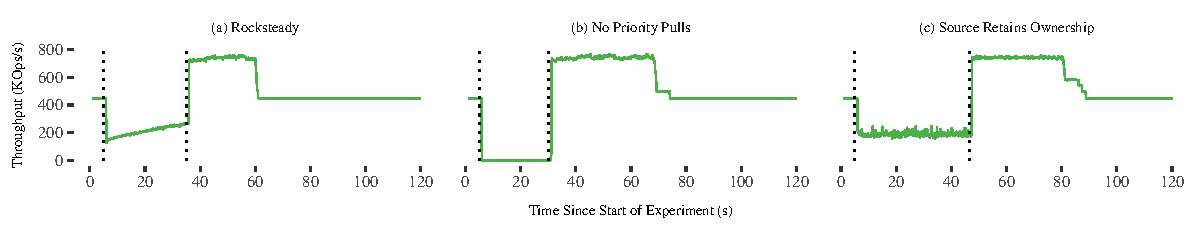
\includegraphics[width=1.0\textwidth]{graphs/rocksteady-throughput.pdf}
\caption{Running total YCSB-B throughput for $($a$)$ Rocksteady, $($b$)$
  Rocksteady with no \priopulls, and $($c$)$ when ownership is left at
  the source throughout the migration. Dotted lines demarcate
  migration start and end.}
\label{fig:running-throughput}
\end{figure}


\begin{figure}[t]
\centering
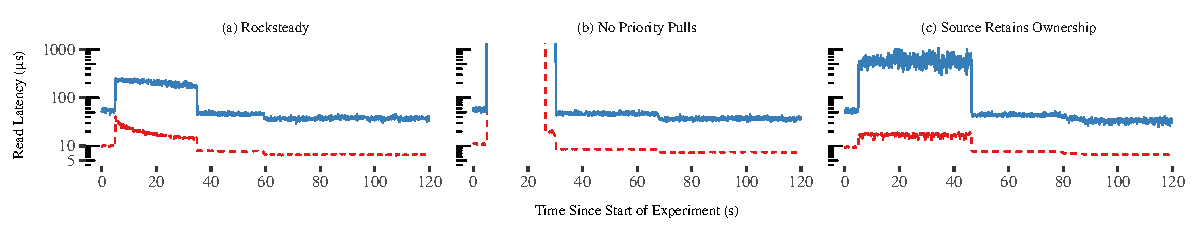
\includegraphics[width=1.0\textwidth]{graphs/rocksteady-latency.pdf}
  \caption{Running median (dashed line) and \nnnth percentile (solid line)
  client-observed access latency on YCSB-B for $($a$)$ Rocksteady,
  $($b$)$ Rocksteady with no \priopulls, and $($c$)$ when ownership is
  left at the source throughout the experiment.}
\label{fig:running-latency}
\end{figure}


All evaluation was done on a 24~server Dell c6220~cluster on the CloudLab
testbed~\cite{cloudlab} (Table~\ref{table:exptconfig}).  RAMCloud is transport
agnostic; it offers RPC over several hardware and transport protocol
combinations.  For these experiments, servers were interconnected with 40~Gbps
Ethernet and Mellanox ConnectX-3 cards; hosts used DPDK~\cite{dpdk} and
the \texttt{mlx4} poll-mode driver for kernel-bypass support.  Each RAMCloud
server used one core solely as a dispatch core to manage the network; it used
12~additional cores as workers to process requests; the remaining
three cores helped prevent interference from background threads. The
dispatch core runs a user-level reliable transport protocol on top of
Ethernet that provides flow control, retransmission, etc.\ without the
overhead of relying on the kernel TCP stack.

%Today, a custom transport protocol (\texttt{Basic
%Transport}\xspace) running over Ethernet using DPDK~\cite{dpdk} is the
%preferred deployment. We used the MLX4 poll mode DPDK driver over the 40
%Gbps NIC port, and allocated two 1~GB hugepages for packet buffers.
%Each node was configured with a dual port Mellanox
%MX354A FDR ConnectX-3 adapter, with both ports flipped to Ethernet mode
%(one at 40 Gbps and the other at 10 Gbps) using Mellanox VPI
%technology~\cite{mellanoxvpi}. Cloudlab's \texttt{r-320}\xspace network
%fabric has two layers of switches: seven on the edge (28 nodes per
%switch), and 2 on the core, with a blocking factor of 3:5:1. We
%allocated all nodes in our cluster under a single edge switch.
%
%For each of our experiments, we configured our cluster to run one
%coordinator, multiple masters, and multiple clients. Each node of our
%cluster always ran only one such RAMCloud instance. We configured our
%RAMCloud masters to allocate 8000~MB of memory for the log, 1 dispatch
%thread, and 7 worker threads. For fault tolerance, we set the
%replication factor to 3 and had every master allocate 32~GB of disk
%space to serve remote replication requests. Additionally, RAMCloud
%supports in-memory buffering of replicated data which can be flushed to
%non-volatile storage in the case of a failure. We set the number of such
%buffers to a value as high as possible to compensate for our small
%experimental cluster and prevent the disks from becoming a bottleneck; a
%real RAMCloud deployment will typically span hundreds of machines and
%hence spray replication requests uniformly across all backups.

%./scripts/clusterperf.py migrateLoaded -T basic+dpdk --workload=YCSB-B --loadPct=90 --seconds=30 --timeout=600 --migratePercentage=50 --size=100 --numObjects=20000000 --masterArgs='--totalMasterMemory=8000 --segmentFrames=4096 --maxCores=8 --maxNonVolatileBuffers=0 -d' --verbose -r 3 --fullSamples --debug --servers=7 --clients=16

To evaluate migration under load, 8~client machines run the YCSB-B~\cite{ycsb}
workload (95\% reads, 5\% writes, keys chosen according to a Zipfian
distribution with $\theta$ = 0.99), which accesses a table on the source
server. The table consists of 300~million 100~B record payloads with 30~B
primary keys constituting 27.9~GB of record data consuming 44.4~GB of in-memory
log on the source. Clients offer a nearly open load to the cluster sufficient to keep
a single server at 80\% (dispatch) load.  While the YCSB load is running, a
migration is triggered that live migrates half of the records from the source
to the target.

Rocksteady was configured to partition the source's key hash space into
8 parts, with each \pull returning 20~KB of data. \pulls were configured
to have the lowest priority in the system. \priopulls returned a batch
of at most 16 records from the
source and were configured
to have the highest priority in the system. The version of Rocksteady
used for the evaluation can be accessed online on github at\linebreak{}
{\small\url{https://github.com/utah-scs/RAMCloud/tree/rocksteady-sosp2017}}.

\subsection{Migration Impact and Ownership}
\label{sec:e2e}
Figures~\ref{fig:running-throughput} and~\ref{fig:running-latency} (a) show
Rocksteady's impact from the perspective of the YCSB clients. Migration
takes 30~s and transfers at 758~MB/s. Throughput drops when ownership is
transferred at the start of migration, since the clients must wait for records
to arrive at the target. As records are being transferred, \nnnth percentile
end-to-end response times start at 250~\us and taper back down to 183~\us as
hot records from \priopulls arrive at the target. After migration, median
response times drop from 10.1~\us to 6.7~\us, since each server's dispatch is under
less load. Likewise, after migration moves enough records, throughput briefly
exceeds the before-migration throughput, since client load is open and some
requests are backlogged.

Figures~\ref{fig:running-throughput} and~\ref{fig:running-latency} (b) show
\priopulls are essential to Rocksteady's design. Without \priopulls, client
requests for a record cannot complete until they are moved by the
\pulls, resulting in requests that cannot complete
until migration is done. Only a small fraction of requests complete
while the migration is ongoing, and throughput is elevated after
migration for a longer period. In practice, this would result in
timeouts for client operations. Migration speed is 19\% faster
(904~MB/s) without \priopulls enabled.

Instead of transferring ownership to the target at the start of migration,
another option is to leave ownership at the source during migration
while synchronously re-replicating migrated data at the target.
Figures~\ref{fig:running-throughput} and~\ref{fig:running-latency} (c) explore
this approach. The main drawback is that it cannot take advantage of the
extra resources that the target provides. Similar to the
case above, source throughput decreases under migration load, and clients
eventually fall behind.  For long migrations, this can lead to client timeouts
%which is evidenced by the increased median access latency while migration
%is ongoing.
in a fully open load, since throughput would drop below offered load for the duration of migration.
Additionally, migration suffers a 27.7\% slowdown
(758~MB/s down to 549~MB/s), and the impact on the \nnnth
percentile access latency is worse than the full Rocksteady protocol
because of the re-replication load generated by the target interfering
with the replication load generated by writes at the source. For larger
RAMCloud clusters, such interference will not be an issue, and one would
expect the \nnnth percentile to be similar to Rocksteady.

\subsection{Load Impact}
\label{sec:eval-load}

\begin{figure}[t]
\centering
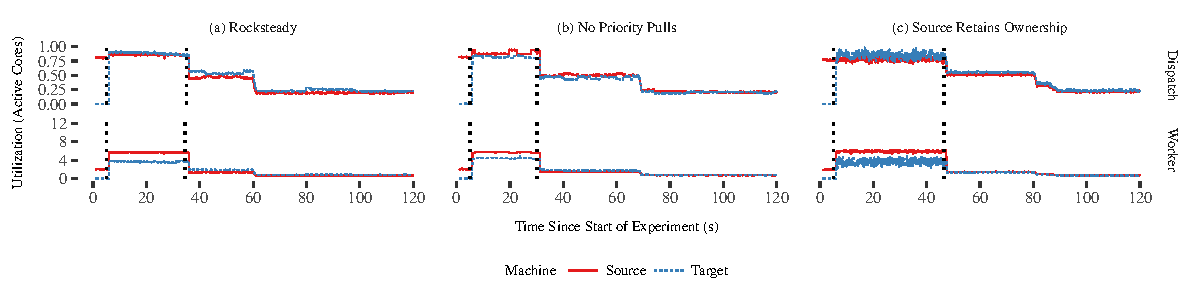
\includegraphics[width=1.0\textwidth]{graphs/running-dispatch-worker}
\caption{Dispatch core and worker core utilization on both source and target
  for $($a$)$ Rocksteady, $($b$)$ Rocksteady with no \priopulls, and
  $($c$)$ when ownership is left at the source throughout the migration.}
\label{fig:load}
\end{figure}


Figure~\ref{fig:load} (a) shows Rocksteady immediately equalizes
dispatch load on the source and target. Worker and dispatch load on the
target jumps immediately when migration starts, offloading the source.
Clients refresh their stale tablet mappings after migration starts.
Dispatch is immediately equalized because
a) exactly half of the table ownership has been shifted to the target, and
b) the migration manager is asynchronous and requires little CPU.

% XXX What causes 11b to increase dispatch load after migration? The decrease
% might be due to the fact that the clients are "stuck" on the target, so they
% backoff on the source too. As the target starts to get the data the clients
% become unstuck and accelerate against the source.

%Dispatch load drops immediately on
%the source, showing that the batching priority pulls have the intended effect.

%Figure~\ref{fig:load} (b) shows that without \priopulls the source and target remain at elevated load longer after migration, since pent up client
%

\begin{figure}[t]
\centering
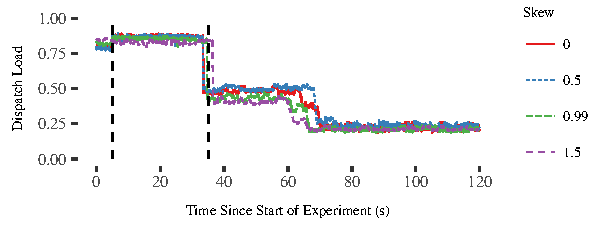
\includegraphics[width=1.0\columnwidth]{graphs/priopull-skew}
\caption{Impact of workload access skew on source-side dispatch load. Batched
  \priopulls hide the extra dispatch load of background \pulls regardless of
  access skew.}
\label{fig:load-skew}
\end{figure}


A key goal of Rocksteady is to shift load quickly from the source to the
target. Most workloads exhibit some skew, but the extent of that skew impacts
Rocksteady's ability to shift load quickly. Figure~\ref{fig:load-skew}
examines the extent to which Rocksteady's effectiveness at reducing client load
is skew dependent. With no skew (uniform access, skew $\theta$ = 0) \priopulls are
sufficient to maintain client access to the tablet, but low request locality
means the full load transfer only proceeds as quickly as the background pulls
can transfer records.  Overall, the results are promising when considering the
source's dispatch load, which is its most scarce resource for typical
read-heavy workloads. Regardless of workload skew, source-side dispatch load
remains relatively flat from the time migration starts until it completes.
This means that  Rocksteady's eager ownership transfer enabled by
batched \priopulls makes up for any extra dispatch load the \pulls place
on the source regardless of the skew.


\subsection{Asynchronous Batched Priority Pulls}
\label{sec:eval-priopulls}

\begin{figure}[t]
\centering
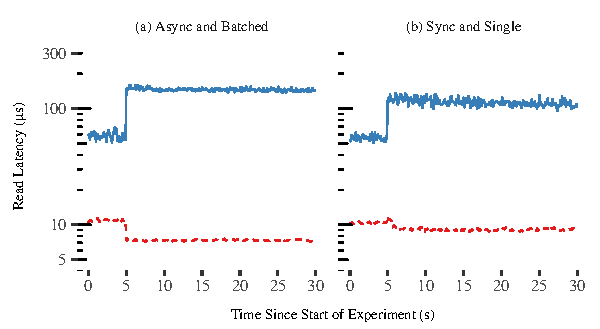
\includegraphics[width=1.0\columnwidth]{graphs/running-latency-only-priority}
  \caption{Median (dashed line) and \nnnth percentile (solid line)
  access latency without background \pulls. Async batched
  \priopulls restore median latency almost immediately compared
  to sync \priopulls.}
\label{fig:batching-lat}
\end{figure}


\begin{figure}[t]
\centering
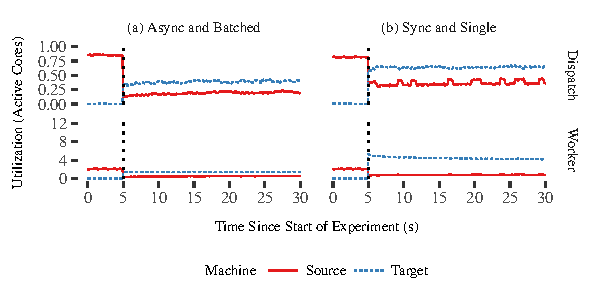
\includegraphics[width=1.0\columnwidth]{graphs/running-dispatch-worker-only-priority}
  \caption{CPU Load with no background \pulls. Asynchronous batched \priopulls
  improve dispatch and worker utilization at both the source and target
  compared to synchronous \pulls that stall target worker cores.}
\label{fig:batching-load}
\end{figure}


Figures~\ref{fig:batching-lat} and~\ref{fig:batching-load} compare
asynchronous batched \priopulls with the na\"{i}ve, synchronous approach
when background \pulls are disabled. The asynchronous
approach doesn't help tail latency:
\nnnth latency stays consistent at 160~\us for the rest of the
experiment, but median access latency drops to 7.4~\us immediately.
On the other hand, the synchronous approach results in
median latency jitter,
primarily due to workers at the target waiting for \priopulls to return, which
can be seen in the increased worker utilization at the target
(Figure~\ref{fig:batching-load}b).  However, \nnnth percentile access latency
is lower than the asynchronous approach since pull responses are sent to
waiting clients immediately.

\priopulls are critical to the goal of
rapidly shifting load away from the source. The headroom thus
obtained can be used to service \pulls at the source thereby allowing
the migration to go as fast as possible. At the same time, \priopulls
help maintain tail latencies by fetching client requested data
on-demand.

\subsection{Pull and Replay Scalability}
\label{sec:eval-replay}

\begin{figure}[t]
\centering
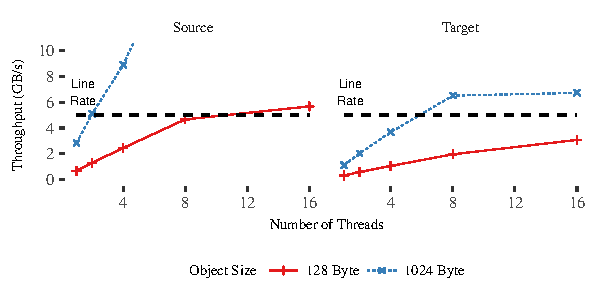
\includegraphics[width=1.0\columnwidth]{graphs/rocksteady-scalability.pdf}
\caption{Source and target parallel migration scalability. Source side
pull logic can process small 128~B objects at 5.7~GB/s. Target side
replay logic can process small 128~B objects at 3~GB/s. For larger
objects, neither side limits migration.}
\label{fig:parallel-replay}
\end{figure}


Parallel and pipelined pulls and replay are key to migration speed that
interleaves with normal case request processing.  The microbenchmark shown in
Figure~\ref{fig:parallel-replay} explores the scalability of the source and
target pull processing logic. In the experiment, the source and target
pull/replay logic was run in isolation on large batches of records to stress
contention and to determine the upper bound on migration speed at both ends
independently.

Overall, both the source and target can process pulls and replays in parallel with
little contention. In initial experiments, performance was limited when the
target replayed records into a single, shared in-memory log, but per-worker side logs
remedy this. Small 128~B records (like those used in the evaluation) are
challenging. They require computing hashes and checksums over many small log
entries on both the source and target. On the target, they also require many
probes into the hash table to insert references, which induces many costly
cache misses. Even so, the source and target can migrate 5.7~GB/s and
3~GB/s
respectively. The source outpaces target replay by 1.8~to~2.4$\times$ on the
same number of cores, so migration stresses the target more than the source.
This works well for scaling out, since the source is likely to be under an
existing load that is being redistributed to a less loaded target. For larger
record sizes, pull/replay logic doesn't limit migration.

